\chapter{Geometry}

\section{Geometric primitives}
	\kactlimport{Point.h}
	\kactlimport{lineDistance.h}
	\kactlimport{SegmentDistance.h}
	\kactlimport{SegmentIntersection.h}
	\kactlimport{lineIntersection.h}
	\kactlimport{sideOf.h}
	\kactlimport{OnSegment.h}
	\kactlimport{linearTransformation.h}
	\kactlimport{LineProjectionReflection.h}
	\kactlimport{Angle.h}

\section{Circles}
	\kactlimport{CircleIntersection.h}
	\kactlimport{CircleTangents.h}
	\kactlimport{CircleLine.h}
	\kactlimport{CirclePolygonIntersection.h}
	\kactlimport{CirclesSumArea.h}
	\kactlimport{circumcircle.h}
	\kactlimport{MinimumEnclosingCircle.h}

\section{Polygons}
	\kactlimport{InsidePolygon.h}
	\kactlimport{PolygonArea.h}
	\kactlimport{PolygonCenter.h}
	\kactlimport{PolygonCut.h}
	\kactlimport{PolygonUnion.h}
	\kactlimport{ConvexHull.h}
	\kactlimport{HullDiameter.h}
	\kactlimport{MinkowskiSum.h}
	\kactlimport{PointInsideHull.h}
	\kactlimport{LineHullIntersection.h}
	\kactlimport{PolygonTangents.h}
	\kactlimport{HalfplaneIntersectionDynamic.h}

\section{Misc. Point Set Problems}
	\kactlimport{ClosestPair.h}
	\kactlimport{ManhattanMST.h}
	\kactlimport{kDTree.h}
	\kactlimport{DelaunayTriangulation.h}
	\kactlimport{FastDelaunay.h}
	\kactlimport{manySegmentsIntersection.h}

\section{Spherical coordinates}

\begin{center}
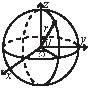
\includegraphics[width=25mm]{content/geometry/sphericalCoordinates}
\end{center}
\[\begin{array}{cc}
x = r\sin\theta\cos\phi & r = \sqrt{x^2+y^2+z^2}\\
y = r\sin\theta\sin\phi & \theta = \textrm{acos}(z/\sqrt{x^2+y^2+z^2})\\
z = r\cos\theta & \phi = \textrm{atan2}(y,x)
\end{array}\]

\section{3D}
	\kactlimport{PolyhedronVolume.h}
	\kactlimport{Point3D.h}
	\kactlimport{3DHull.h}
	\kactlimport{sphericalDistance.h}
	\kactlimport{SpheresIntersection.h}
